\chapter{Arhitektura i dizajn sustava}
		
	
		Arhitektura sustava je izvedena u obliku web aplikacije kojoj korisnik pristupa koristeći web preglednik. Web preglednik omogućuje korisniku pregled web-stranica i multimedijskog sadržaja na njima. Postoje razni web preglednici za različite operacijske sustave te ovaj pristup omogućava lak i širok pristup aplikaciji bez potrebe za dodatnim preuzimanjem programske podrške od strane korisnika.
	\par Za razvoj aplikacije koristimo programski jezik Python, HTML, JavaScript i CSS. Koristimo razvojno okruženje Django koje smo odabrali zbog njegove jednostavnosti, modularnosti te upoznatosti tima s razvojem u toj okolini.
Korisnik vrši interakcije sa aplikacijom preko Django predložaka. Predlošci (eng. \textit{templates}) sadrže strukturu potrebnu za dinamičko generiranje HTML stranice i prikaz iste korisniku.



	\begin{figure}[H]
						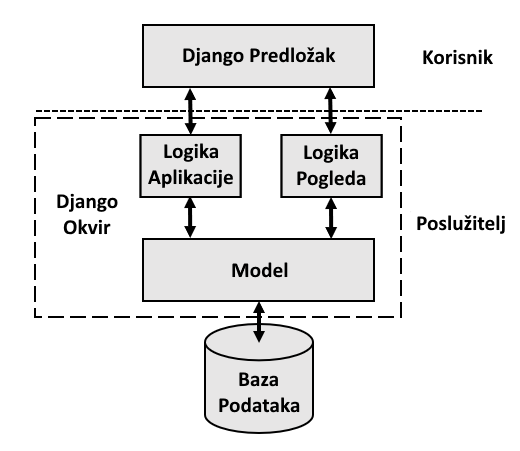
\includegraphics[scale=0.9]{dijagrami/django.png} 
						\centering
						\caption{Dijagram načina rada Djanga}
						\label{fig:dijagramRadaDjanga}
					\end{figure}

		Django predlošci su jedan od sastavnih dijelova radnog okvira Django. Django funkcionira na MVT principu rada, koji je strukturno vrlo sličan modelu MVC.\newline MVT model se sastoji od:
\begin{itemize}
		\item 	\textbf{Model} - objekti u Pythonu koji definiraju strukturu podataka aplikacije i omogućavaju dodavanje, brisanje, mijenjanje i dohvaćanje podataka iz baze podataka.
		\item 	\textbf{View (pogled)} - funkcije koje sluze za obradu HTTP zahtjeva i generiranje HTTP odziva. Pogledi pristupaju podatcima potrebnima za odrađivanje zahtjeva uz pomoć modela, a za formatiranje i prikaz  dohvaćenih podataka koriste predloške.
		\item 	\textbf{Template (predložak)} - definira strukturu prikaza podataka neke datoteke (npr. HTML). Pogledi mogu dinamički generirati HTML stranice uz pomoć predložaka i popuniti ih s podacima dohvaćenih putem modela. 
				
	\end{itemize}

		\begin{figure}[H]
						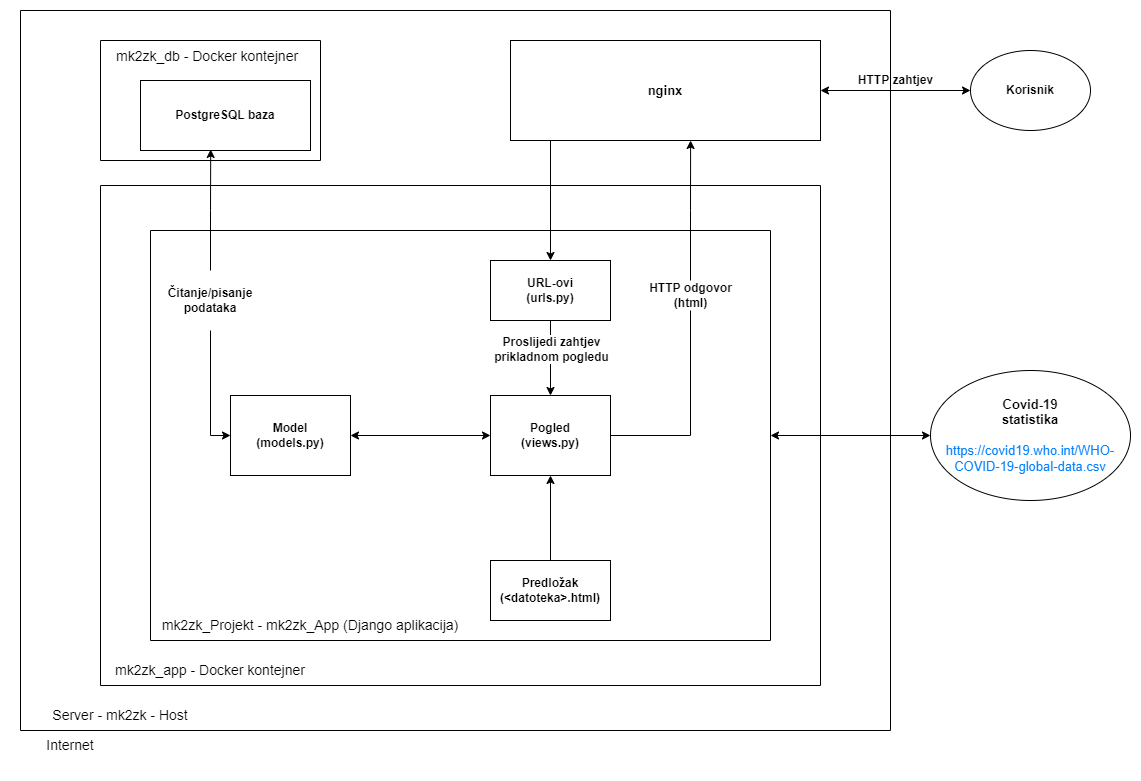
\includegraphics[scale=0.9]{dijagrami/django_mvt.png} 
						\centering
						\caption{Dijagram principa rada MVT}
						\label{fig:dijagramRadaMVT}
					\end{figure}

		

				
		\section{Baza podataka}
			
			\textbf{\textit{dio 1. revizije}}\\
			
			Baze podataka neizostavan su dio razvoja programske potpore jer danas gotova svaka domena primjene djeluje mnoštvom podataka koje treba pohraniti na organiziran način kako bi se efikasno dohvaćali, mijenjali i nadopunjavali. Za upravljanje bazom podataka mogu se koristiti različiti sustavi koji obavljaju optimiranje upita i omogućuju rukovanje podacima. Mi smo odlučili koristiti PostgreSQL koji nam je bio preporučen na kolegiju Baze podataka. \newline Iako stvarni svijet ne možemo prikazati sa svim detaljima, relacijski nam model baze podataka omogućuje vjeran prikaz stvarnosti pomoću relacija u koje pohranjujemo vrijednosti odabranih atributa koji su vezani uz entitete bitne za domenu primjene. Formalno gledano relacija, odnosno instanca relacije, definirana na relacijskoj shemi je skup n-torki, a neformalno možemo reći da je to imenovana dvodimenzionalna tablica. Atributi su imenovani stupci te tablice. ER (\textit{Entity-Relationship}) model podataka zadržava dobra svojstva relacijskog modela, a uz to omogućuje eksplicitni prikaz semantičkih informacija vezanih uz veze (odnose) između entiteta. ER dijagram prikazuje kako su entiteti našeg sustava povezani. Pri preslikavanju ER modela u relacijski model, entiteti i veze postaju entiteti (relacije) te se sheme s jednakim ključevima zamjene njihovom unijom.
		Baza podataka ove aplikacije sastoji se od sljedećih entiteta:
		\begin{packed_item}
			\item Korisnik
			\item Rad
			\item Autor
			\item AutorRad
			\item Sekcija
			\item Uloga
			\item Konferencija
			\item DodatnoPoljeObrasca
			\item TipPoljeObrasca
			\item DodatniPodatak 
			\item Recenzija
			\item Ocjena
			\item Ustanova
		\end{packed_item}
		
			\subsection{Opis tablica}
			

				\textbf{Korisnik}
				Ovaj entitet sadržava sve važne informacije (atribute) o svim korisnicima aplikacije: korisničko ime, e-mail, lozinku, ime, prezime te ulogu korisnika u sustavu. Atributi token i potvrdioPrijava služe kako bi se za sudionike i recenzente provjerilo jesu li potvrdili prijavu (nakon čega se mogu prijaviti u sustav). Atribut sudionikID je svojstven korisnicima koji su sudionici, a atribut odobren i sifSekcija je svojstven recenzentima. Ovaj entitet je u vezi \begin{packed_item} 
					\item Many-to-One s entitetom Ustanova preko atributa ID
					\item Many-to-One s entitetom Sekcija preko atributa ID
					\item Many-to-One s entitetom Uloga preko atributa ID
					\item One-to-Many s entitetom Recenzija preko atributa ID (Recenzija.recezentID)
					\item Many-to-Many s entitetom DodatnoPoljeObrasca preko atributa ID (DodatniPodatak.korisnikID; ta je veza na ER dijagramu imenovana kao DodatniPodatak pa se može reći da je entitet Korisnik u vezi One-to-Many s entitetom DodatniPodatak preko atributa ID)
					\item One-to-Many s entitetom Rad preko atributa ID (Rad.prijavioID)
				\end{packed_item}
				\begin{longtblr}[
					label=none,
					entry=none
					]{
						width = \textwidth,
						colspec={|X[7,l]|X[6, l]|X[20, l]|}, 
						rowhead = 1,
					} %definicija širine tablice, širine stupaca, poravnanje i broja redaka naslova tablice
					\hline \multicolumn{3}{|c|}{\textbf{Korisnik}}	 \\ \hline[3pt]
					\SetCell{LightGreen}ID & INT	&  jedinstveni brojčani identifikator	\\ \hline
					korisnickoIme	& VARCHAR & korisnički identifikator  kojeg korisnik koristi pri prijavi u sustav	\\ \hline 
					email & VARCHAR & adresa e-pošte korisnika  \\ \hline 
					lozinka & VARCHAR & hash lozinke  \\ \hline 
					ime & VARCHAR	&  	ime korisnika	\\ \hline 
					prezime & VARCHAR & prezime korisnika  \\ \hline 
					sudionikID & INT & jedinstvena oznaka sudionika (ID\_XXXX, 
					pri čemu je XXXX redni broj prijave)\\ \hline 
					odobren & BOOLEAN & oznaka je li predsjedavajući konferencije odobrio recenzenta\\ \hline 
					token & VARCHAR & link koji se šalje sudionicima i recenzentima na e-mail kako bi klikom na njega potvrdili svoju prijavu  \\ \hline
					potvrdioPrijava & BOOLEAN & oznaka je li korisnik (sudionik/recenzent) potvrdio svoju prijavu\\ \hline  
					\SetCell{LightBlue} sifUstanova	& INT & jedinstvna brojčana oznaka matične ustanove korisnika (Ustanova.ID)  	\\ \hline 
					\SetCell{LightBlue} sifSekcija	& INT & jedinstvena brojčana oznake sekcije (Sekcija.ID) u kojoj je
					recenzent odabrao recenzirati radove	\\ \hline 
					\SetCell{LightBlue} ulogaKorisnik	& INT & oznaka korisnikove uloge u sustavu (Uloga.ID) \\ \hline 
				\end{longtblr}
				\textbf{Ustanova} Ovaj entitet predstavlja ustanove (poduzeća ili institucije) kojima pripadaju prijavljeni sudionici i recenzenti. Atributi ovog entiteta su: ID, naziv, grad, država i adresa ustanove. Entitet je u vezi
				\begin{packed_item}
					\item One-to-Many s entitetom Korisnik preko atributa sifUstanova (jedinstveni brojčani identifikator ustanove; Korisnik.sifUstanova).	
				\end{packed_item} 
				\begin{longtblr}[
					label=none,
					entry=none
					]{
						width = \textwidth,
						colspec={|X[6,l]|X[6, l]|X[20, l]|}, 
						rowhead = 1,
					} %definicija širine tablice, širine stupaca, poravnanje i broja redaka naslova tablice
					\hline \multicolumn{3}{|c|}{\textbf{Ustanova}}	 \\ \hline[3pt]
					\SetCell{LightGreen}ID & INT	&  jedinstveni brojčani identifikator	\\ \hline
					naziv	& VARCHAR &   naziv ustanove	\\ \hline 
					grad & VARCHAR & grad u kojem je ustanova  \\ \hline 
					drzava & VARCHAR	&  država u kojoj je ustanova		\\ \hline 
					adresa & VARCHAR	&  adresa ustanove		\\ \hline 
					
				\end{longtblr}
				\textbf{Uloga}
				Ovaj entitet predstavlja ulogu koju korisnik sustava može imati. U ovom sustavu razlikujemo 4 uloge: sudionik, administrator, predsjedavajući konferencije i recenzent. Svaki korisnik ima samo jednu ulogu. Atributi ovog entiteta su: ID i naziv uloge. Entitet je u vezi:
				\begin{packed_item}
					\item One-to-Many s entitetom Korisnik preko atributa ID (Korisnik.ulogaKorisnik)
				\end{packed_item}
				\begin{longtblr}[
					label=none,
					entry=none
					]{
						width = \textwidth,
						colspec={|X[6,l]|X[6, l]|X[20, l]|}, 
						rowhead = 1,
					} %definicija širine tablice, širine stupaca, poravnanje i broja redaka naslova tablice
					\hline \multicolumn{3}{|c|}{\textbf{Uloga}}	 \\ \hline[3pt]
					\SetCell{LightGreen}ID & INT	& jedinstveni brojčani identifikator	\\ \hline
					naziv	& VARCHAR &   naziv uloge	\\ \hline 
					
				\end{longtblr}
				
				\textbf{Ocjena}
				Ovaj entitet predstavlja ocjenu kojom recenzenti mogu ocijeniti neki rad. Početno, u sustavu razlikujemo 4 ocjene (4 jedinstvena brojčana identifikatora) čije se značenje razlikuje (prihvaćanje rada, prihvaćanje rada uz manju doradu, prihvaćanje rada uz veću doradu, neprihvaćanje rada). Ovaj entitet je u vezi 	\begin{packed_item} 
					\item One-to-Many s entitetom Recenzija preko atributa ID (Recenzija.ocjena)
				\end{packed_item}
				\begin{longtblr}[
					label=none,
					entry=none
					]{
						width = \textwidth,
						colspec={|X[6,l]|X[6, l]|X[20, l]|}, 
						rowhead = 1,
					} %definicija širine tablice, širine stupaca, poravnanje i broja redaka naslova tablice
					\hline \multicolumn{3}{|c|}{\textbf{Ocjena}}	 \\ \hline[3pt]
					\SetCell{LightGreen}ID & INT	& jedinstveni brojčani identifikator	\\ \hline
					znacenje	& VARCHAR &   značenje odabrane ocjene	\\ \hline 
					
				\end{longtblr}
				\textbf{Sekcija}
				Ovaj entitet predstavlja sekcije na konferenciji. Na znanstvenoj konferenciji koju modeliramo može biti više sekcija, recenzent recenzira radove unutar jedne sekcije, a svaki rad pripada točno jednoj sekciji. Identifikator entiteta je atribut ID. Entitet sadrži informaciju o nazivu sekcije i u vezi je
				\begin{packed_item}
					\item Many-to-One s entitetom Konferencija preko atributa ID
					\item One-to-Many s entitetom Korisnik preko atributa ID (Korisnik.sifSekcija)
					\item One-to-Many s entitetom Rad preko atributa ID (Rad.sifSekcija)
				\end{packed_item} 
				\begin{longtblr}[
					label=none,
					entry=none
					]{
						width = \textwidth,
						colspec={|X[7,l]|X[6, l]|X[20, l]|}, 
						rowhead = 1,
					} %definicija širine tablice, širine stupaca, poravnanje i broja redaka naslova tablice
					\hline \multicolumn{3}{|c|}{\textbf{Sekcija}}	 \\ \hline[3pt]
					\SetCell{LightGreen}ID & INT	&  	jedinstveni brojčani identifikator	\\ \hline
					naziv	& VARCHAR &   naziv konferencije	\\ \hline 
					\SetCell{LightBlue} sifKonferencija	& INT &   jedinstveni brojčani identifikator konferencije (Konferencija.ID)	\\ \hline
					
				\end{longtblr}
				\textbf{Konferencija}
				Ovaj entitet sadrži važne informacije o znanstvenoj konferenciji koju modeliramo. Atributi su: identifikator konferencije (ID), naziv konferencije, opis, datum održavanja, rok za prijave, rok za administracijske promjene, rok za recenzente. Entitet je u vezi
				\begin{packed_item}
					\item One-to-Many s entitetom Sekcija preko atributa ID (Sekcija.sifKonferencija)
					
				\end{packed_item}
				\begin{longtblr}[
					label=none,
					entry=none
					]{
						width = \textwidth,
						colspec={|X[8,l]|X[6, l]|X[20, l]|}, 
						rowhead = 1,
					} %definicija širine tablice, širine stupaca, poravnanje i broja redaka naslova tablice
					\hline \multicolumn{3}{|c|}{\textbf{Konferencija}}	 \\ \hline[3pt]
					\SetCell{LightGreen}ID & INT	& jedinstveni brojčani identifikator	\\ \hline
					naziv	& VARHCAR & naziv konferencije  	\\ \hline 
					opis & VARCHAR &  opis konferencije \\ \hline
					datum & DATE &  datum održavanja konferencije \\ \hline 
					rokPrijava & TIMESTAMP &  rok za prijavu na konferenciju i učitanje rada u sustav \\ \hline 
					rokAdmin & TIMESTAMP &  rok do kojeg administrator može mijenjati obrazac za prijavu \\ \hline 
					rokRecenzent & TIMESTAMP &  rok do kojeg recenzenti mogu (trebaju) obaviti recenziju radova \\ \hline
					pocetakRecenzent & TIMESTAMP & vremenski trenutak od kojeg recenzenti mogu recenzirati radove  \\ \hline
					pocetakPrijava & TIMESTAMP & vremenski trenutak od kojeg se sudionici i recenzenti mogu početi prijavljivati na konferenciju  \\ \hline
					
					
				\end{longtblr}
				
				\textbf{DodatnoPoljeObrasca} Ovaj entitet sadrži informacije o dodatnim poljima obrasca koja se nude administratoru pri definiranju obrasca za prijavu na konferenciju. Atributi su: ID (jedinstveni identifikator), naziv polja, tip polja, oznake obavezno i prisutno. Entitet je u vezi
				\begin{packed_item}
					\item Many-to-One s entitetom TipPoljeObrasca preko atributa ID
					\item Many-to-Many s entitetom Korisnik preko atributa ID \newline (DodatniPodatak.poljeObrascaID; ta je veza na ER dijagramu imenovana kao DodatniPodatak pa se može reći da je entitet DodatnoPoljeObraca u vezi One-to-Many s entitetom DodatniPodatak preko atributa ID)
				\end{packed_item} 
				\begin{longtblr}[
					label=none,
					entry=none
					]{
						width = \textwidth,
						colspec={|X[6,l]|X[6, l]|X[20, l]|}, 
						rowhead = 1,
					} %definicija širine tablice, širine stupaca, poravnanje i broja redaka naslova tablice
					\hline \multicolumn{3}{|c|}{\textbf{DodatnoPoljeObrasca}}	 \\ \hline[3pt]
					\SetCell{LightGreen}ID & INT	&  jedinstveni brojčani identifikator 	\\ \hline
					ime	& VARCHAR & ime dodatnog polja obrasca  	\\ \hline 
					\SetCell{LightBlue}tipPolje	& INT & tip dodatnog polja obrasca  	\\ \hline 
					obavezno	& BOOLEAN & oznaka je li polje obavezno polje obrasca	\\ \hline
					prisutno	& BOOLEAN & oznaka treba li polje biti prisutno u obrascu	\\ \hline
					
				\end{longtblr}
				\textbf{TipPoljeObrasca}
				Ovaj entitet sadrži informacije o tipovima polja obrasca koja se nude administratoru pri definiranju dodatnih polja obrasca za prijavu. Početno, u sustavu postoje tri tipa polja obrasca: text, number i date. Atributi ovog entiteta su: ID (jedinstveni identifikator) i naziv tipa. Entitet je u vezi
				\begin{packed_item} 
					\item One-to-Many s entitetom DodatnoPoljeObrasca preko atributa ID (DodatnoPoljeObrasca.tipPolja)
					
				\end{packed_item}
				\begin{longtblr}[
					label=none,
					entry=none
					]{
						width = \textwidth,
						colspec={|X[12,l]|X[6, l]|X[20, l]|}, 
						rowhead = 1,
					} %definicija širine tablice, širine stupaca, poravnanje i broja redaka naslova tablice
					\hline \multicolumn{3}{|c|}{\textbf{TipPoljeObrasca}}	 \\ \hline[3pt]
					\SetCell{LightGreen}ID & INT	&  jedinstveni brojčani identifikator	\\ \hline
					
					nazivTipa	& VARCHAR & naziv tipa polja obrasca\\ \hline 
					
				\end{longtblr}
				\textbf{Recenzija} Ovaj entitet sadrži informacije o recenzijama predanih radova. Atributi su: ID, ocjena, obrazloženje, recenzentID i sifRad. Entitet je u vezi:
				\begin{packed_item}
					\item Many-to-One s entitetom Ocjena preko atributa ID
					\item Many-to-One s entitetom Korisnik preko atributa ID
					\item One-to-One s entitetom Rad preko atributa ID
				\end{packed_item}  
				\begin{longtblr}[
					label=none,
					entry=none
					]{
						width = \textwidth,
						colspec={|X[6,l]|X[6, l]|X[20, l]|}, 
						rowhead = 1,
					} %definicija širine tablice, širine stupaca, poravnanje i broja redaka naslova tablice
					\hline \multicolumn{3}{|c|}{\textbf{Recenzija}}	 \\ \hline[3pt]
					\SetCell{LightGreen}ID & INT	&  jedinstveni brojčani identifikator	\\ \hline
					\SetCell{LightBlue}ocjena	& INT &   odabrana ocjena rada (Ocjena.ID)	\\ \hline 
					obrazlozenje & VARCHAR & obrazloženje za odabranu ocjenu rada\\ \hline 
					\SetCell{LightBlue} recenzentID	& INT & jedinstveni identifikator recenzenta (Korisnik.ID)	\\ \hline 
					\SetCell{LightBlue} sifRad	& INT &   jedinstveni identifikator rada koji se recenzira (Rad.ID)	\\ \hline 
				\end{longtblr}
				\textbf{Rad}
				Ovaj entitet sadrži informacije o prijavljenim radovima: ID rada, naslov, poveznicu s pdf dokumentom, je li rad recenziran, u koju je sekciju prijavljen i koji korisnik ga je prijavio. Entitet je u vezi:
				\begin{packed_item}
					\item One-to-One s entitetom Recenzija preko atributa ID (Recenzija.sifRad)
					\item Many-to-One s entitetom Sekcija preko atributa ID
					\item Many-to-One s entitetom Korisnik preko atributa ID
					\item Many-to-Many s entitetom Autor preko atributa ID (ta je veza u ER dijagramu prikazana kao entitet AutorRad pa možemo reći da je entitet Rad u vezi One-to-Many s entitetom AutorRad preko atributa ID(AutorRad.sifRad))
				\end{packed_item}
				\begin{longtblr}[
					label=none,
					entry=none
					]{
						width = \textwidth,
						colspec={|X[6,l]|X[6, l]|X[20, l]|}, 
						rowhead = 1,
					} %definicija širine tablice, širine stupaca, poravnanje i broja redaka naslova tablice
					\hline \multicolumn{3}{|c|}{\textbf{Rad}}	 \\ \hline[3pt]
					\SetCell{LightGreen}ID & INT	&  	jedinstveni brojčani identifikator	\\ \hline
					naslov	& VARCHAR &   naslov rada	\\ \hline 
					pdf & VARCHAR &  poveznica s pdf dokumentom rada \\ \hline 
					recenziran & BOOLEAN	& oznaka je li rad recenziran 		\\ \hline 
					\SetCell{LightBlue} sifSekcija	& INT & jedinstveni brojčani identifikator sekcije u koju je rad prijavljen(Sekcija.ID)   	\\ \hline 
					\SetCell{LightBlue} prijavioID	& INT & jedinstveni brojčani identifikator sudionika koji je prijavio rad (Korisnik.ID) \\\hline 
				\end{longtblr}
				\textbf{Autor}
				Ovaj entitet sadrži važne informacije o autorima predanih radova. Atributi su: ID, ime, prezime i e-mail.
				Entitet je u vezi
				\begin{packed_item}
					\item Many-to-Many s entitetom Rad preko atributa ID (ta je veza u ER dijagramu prikazana kao entitet AutorRad pa možemo reći da je entitet Autor u vezi One-to-Many s entitetom AutorRad preko atributa ID (AutorRad.sifAutor))
				\end{packed_item}
				\begin{longtblr}[
					label=none,
					entry=none
					]{
						width = \textwidth,
						colspec={|X[6,l]|X[6, l]|X[20, l]|}, 
						rowhead = 1,
					} %definicija širine tablice, širine stupaca, poravnanje i broja redaka naslova tablice
					\hline \multicolumn{3}{|c|}{\textbf{Autor}}	 \\ \hline[3pt]
					\SetCell{LightGreen}ID & INT	&  jedinstveni brojčani identifikator	\\ \hline
					ime	& VARCHAR & autorovo ime	\\ \hline 
					prezime	& VARCHAR &   autorovo prezime	\\ \hline
					email & VARCHAR & e-mail autora  \\ \hline 
					
				\end{longtblr}
				\textbf{AutorRad}
				Ovaj entitet prikazan na ER dijagramu predstavlja Many-to-Many vezu između entiteta Autor i entiteta Rad. Kad bismo tu vezu prikazali kao entitet primarni ključ bi bio kompozitni ključ: ID autora i ID rada. Atribut veze je naznakaOZK na temelju koje se zna je li autor označen kao osoba za kontakt pri prijavi tog rada.
				Može se reći da je entitet u vezi:
				\begin{packed_item}
					\item Many-to-One s entitetom Autor preko atributa sifAutor
					\item Many-to-One s entitetom Rad preko atributa sifRad
				\end{packed_item}
				
				\begin{longtblr}[
					label=none,
					entry=none
					]{
						width = \textwidth,
						colspec={|X[6,l]|X[6, l]|X[20, l]|}, 
						rowhead = 1,
					} %definicija širine tablice, širine stupaca, poravnanje i broja redaka naslova tablice
					\hline \multicolumn{3}{|c|}{\textbf{AutorRad}}	 \\ \hline[3pt]
					\SetCell{LightGreen}sifRad & INT	&  jedinstveni brojčani identifikator rada	\\ \hline
					\SetCell{LightGreen}sifAutor& INT	&  kedinstveni brojčani identifikator autora	\\ \hline
					naznakaOZK & BOOLEAN	& naznaka je li autor označen kao osoba za kontakt za navedeni rad 		\\ \hline 
					
					
				\end{longtblr}
			\textbf{DodatniPodatak} Ovaj entitet prikazan na ER dijagramu predstavlja Many-to-Many vezu između entiteta Korisnik i entiteta DodatnoPoljeObrasca. Kad bismo tu vezu prikazali kao entitet, primarni bi ključ bio kompozitni ključ: ID korisnika i ID dodatnog polja obrasca. Dodatni atribut ove veze (entiteta) jest podatak - podatak kojeg korisnik unosi u dodatno polje obrasca pri prijavi na konferenciju. Može se reći da je entitet u vezi 
				\begin{packed_item}
					\item Many-to-One s entitetom Korisnik preko atributa korisnikID
					\item Many-to-One s entitetom DodatnoPoljeObrasca preko atributa poljeObrascaID
				\end{packed_item}
				
				\begin{longtblr}[
					label=none,
					entry=none
					]{
						width = \textwidth,
						colspec={|X[7,l]|X[6, l]|X[20, l]|}, 
						rowhead = 1,
					} %definicija širine tablice, širine stupaca, poravnanje i broja redaka naslova tablice
					\hline \multicolumn{3}{|c|}{\textbf{DodatniPodatak}}	 \\ \hline[3pt]
					\SetCell{LightGreen}korisnikID & INT	& jedinstveni brojčani identifikator korisnika 	\\ \hline
					\SetCell{LightGreen}poljeObrascaID& INT	&  jedinstveni brojčani identifikator dodatnog polja obrasca	\\ \hline
					podatak & VARCHAR	&  podatak koji je korisnik unio u to polje obrasca	\\ \hline 
					
				\end{longtblr}
				
				
			\newpage
			\subsection{Dijagram baze podataka}
			
				\begin{figure}[H]
					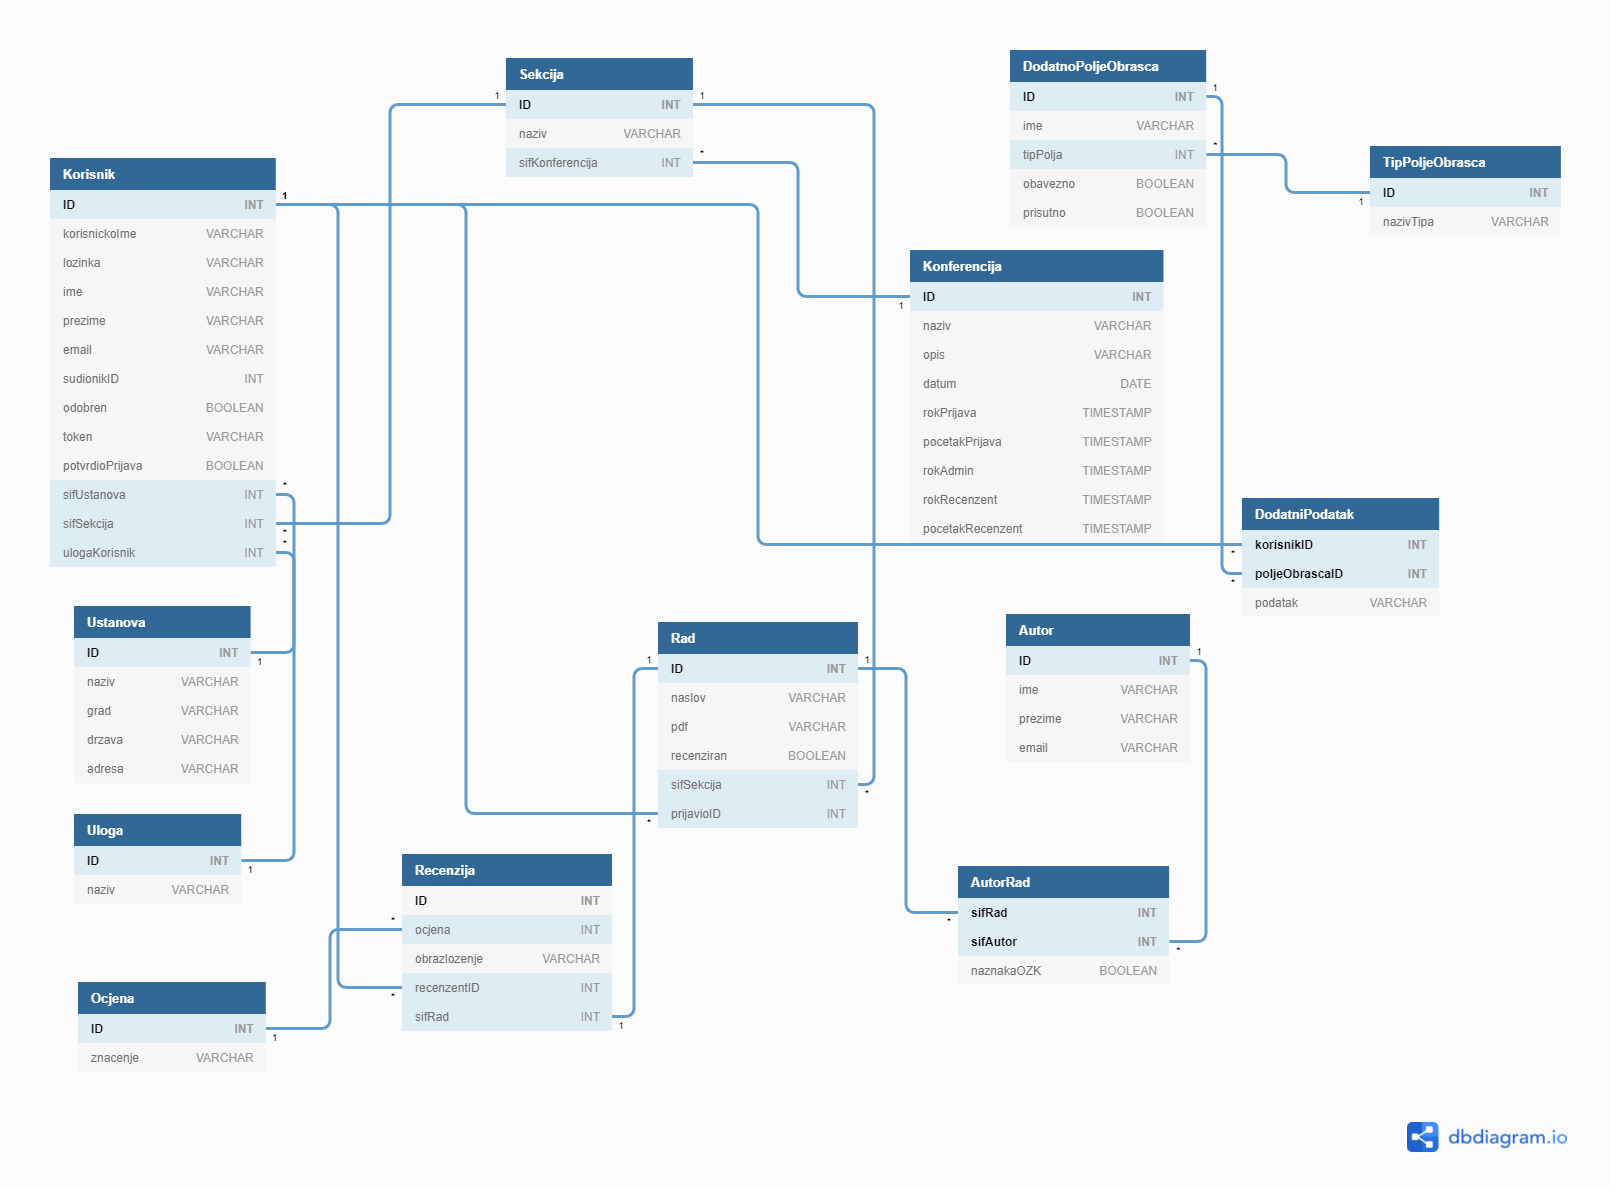
\includegraphics[width= 15 cm, keepaspectratio]{dijagrami/ZK-ER-DIJAGRAM.png} 
					\centering
					\caption{ER dijagram baze podataka}
					\label{fig:ERdijagram}
				\end{figure}
			\eject
			
			
		\section{Dijagram razreda}
		
			\textit{Potrebno je priložiti dijagram razreda s pripadajućim opisom. Zbog preglednosti je moguće dijagram razlomiti na više njih, ali moraju biti grupirani prema sličnim razinama apstrakcije i srodnim funkcionalnostima.}\\
			
			\textbf{\textit{dio 1. revizije}}\\
			
			\textit{Prilikom prve predaje projekta, potrebno je priložiti potpuno razrađen dijagram razreda vezan uz \textbf{generičku funkcionalnost} sustava. Ostale funkcionalnosti trebaju biti idejno razrađene u dijagramu sa sljedećim komponentama: nazivi razreda, nazivi metoda i vrste pristupa metodama (npr. javni, zaštićeni), nazivi atributa razreda, veze i odnosi između razreda.}\\
			
			\textbf{\textit{dio 2. revizije}}\\			
			
			\textit{Prilikom druge predaje projekta dijagram razreda i opisi moraju odgovarati stvarnom stanju implementacije}
			
			
			
			\eject
		
		\section{Dijagram stanja}
			
			
			\textbf{\textit{dio 2. revizije}}\\
			
			\textit{Potrebno je priložiti dijagram stanja i opisati ga. Dovoljan je jedan dijagram stanja koji prikazuje \textbf{značajan dio funkcionalnosti} sustava. Na primjer, stanja korisničkog sučelja i tijek korištenja neke ključne funkcionalnosti jesu značajan dio sustava, a registracija i prijava nisu. }
			
			
			\eject 
		
		\section{Dijagram aktivnosti}
			
			\textbf{\textit{dio 2. revizije}}\\
			
			 \textit{Potrebno je priložiti dijagram aktivnosti s pripadajućim opisom. Dijagram aktivnosti treba prikazivati značajan dio sustava.}
			
			\eject
		\section{Dijagram komponenti}
		
			\textbf{\textit{dio 2. revizije}}\\
		
			 \textit{Potrebno je priložiti dijagram komponenti s pripadajućim opisom. Dijagram komponenti treba prikazivati strukturu cijele aplikacije.}